\documentclass[a4paper,12pt,twoside,openright]{report}

\usepackage[pdfborder={0 0 0}]{hyperref}    % turns references into hyperlinks
\usepackage[margin=25mm]{geometry}  % adjusts page layout
\usepackage{graphicx}  % allows inclusion of PDF, PNG and JPG images
\usepackage{verbatim}
\usepackage{pdfpages}  % to embed proposal at the end of the dissertation
\usepackage{textcomp}
\usepackage{appendix}

\renewcommand{\baselinestretch}{1.1}    % adjust line spacing to make
% more readable

\begin{document}
	
	%%%%%%%%%%%%%%%%%%%%%%%%%%%%%%%%%%%%%%%%%%%%%%%%%%%%%%%%%%%%%%%%%%%%%%%%
	% Title
	
	
	\pagestyle{empty}
	
	\rightline{\LARGE \textbf{Peter Lotts}}
	
	\vspace*{60mm}
	\begin{center}
		\Huge
		\textbf{Adding network subsystem provenance collection to CADETS} \\[5mm]
		Computer Science Tripos -- Part II \\[5mm]
		Downing College \\[5mm]
		\today  % today's date
	\end{center}
	
	%%%%%%%%%%%%%%%%%%%%%%%%%%%%%%%%%%%%%%%%%%%%%%%%%%%%%%%%%%%%%%%%%%%%%%%%%%%%%%
	% Proforma, table of contents and list of figures
	
	\pagestyle{plain}
	
	\chapter*{Proforma}
	
	{\large
		\begin{tabular}{ll}
			Name:               & \bf Peter Lotts                       \\
			College:            & \bf Downing College                     \\
			Project Title:      & \bf Adding network subsystem provenance \\
								& \bf collection to CADETS \\
			Examination:        & \bf Computer Science Tripos -- Part II, 2018  \\
			Word Count:         & \bf tbc\footnotemark[1]  \\
			Project Originator: & Dr R.~Sohan                    \\
			Supervisor:         & Dr G.~Jenkinson                    \\ 
		\end{tabular}
	}
	\footnotetext[1]{This word count was computed at [date]	by the provided online tool at \texttt{URL}
	}
	\stepcounter{footnote}
	
	
	\section*{Original Aims of the Project}
	
	To provide additional metadata collection tools for network packets to the Computer Laboratory's existing CADETS project. This will be provided by tracking individual packets as they flow through the network stack of the FreeBSD\footnote{\texttt{http://www.freebsd.org/}} kernel, and making information regarding memory locations used and the time taken by each layer to process a given packet available to DTrace\footnote{\texttt{http://dtrace.org/}}. DTrace is a generic Dynamic Tracing framework which is the primary data collection tool used by the CADETS project to bring kernel data into userspace for analysis. The performance impact of the project on network packet delivery is to be evaluated.
	
	
	\section*{Work Completed}
	
	\textit{What we actually did.}
	
	\section*{Special Difficulties}
	
	None. [We hope!!]
	
	\newpage
	\section*{Declaration Of Originality}
	
	I, Peter Lotts of Downing College, being a candidate for Part II of
	the Computer Science Tripos, hereby declare
	that this dissertation and the work described in it are my own work,
	unaided except as may be specified below, and that the dissertation
	does not contain material that has already been used to any substantial
	extent for a comparable purpose.
	
	\bigskip
	\leftline{Signed [signature]}
	
	\medskip
	\leftline{Date [date]}
	
	\tableofcontents
	
	\listoffigures
	
	%%%%%%%%%%%%%%%%%%%%%%%%%%%%%%%%%%%%%%%%%%%%%%%%%%%%%%%%%%%%%%%%%%%%%%%
	% now for the chapters
	
	\pagestyle{headings}
	
	\chapter{Introduction}
	
	\section{Use Case}
	
	In this project I am evaluating the application of fine-grained tracing within the network stack of the FreeBSD kernel by implementing additional statically defined DTrace probes which are able to provide a platform for both security and performance analysis.
	
	The security aspect of the tool is most useful in combating Advanced Persistent Threats (APTs)\cite{Tankard-APT}, where the attacker slowly infiltrates the target system, hiding out of sight until they can exploit knowledge gained to access the enterprise’s internal network. This may allow the attacker to extract sensitive data from databases in such a way that the access is very hard to distinguish from normal access. Eventually, it is likely that the malware will make a mistake and trigger an indicator of compromise to be observed by administrators, but by then it is difficult to tell what data the malware has seen.
	
	The Computer Laboratory has a project which is trying to combat this by building CADETS\cite{CADETS-main} on top of the FreeBSD operating system, which tracks the provenance of data by collecting metadata from computers all over the network about what processes act on what data and when. This metadata is then collected in a distributed database, where it can be analysed to trace data flows throughout the computer system.
	
	My project adds support for collecting metadata on network packets as they flow through the kernel	network stack. The data collected will allow users of CADETS to seek out suspicious activity which may be being used to attack a system, and will be able to provide a list of locations in kernel memory where packet data were stored. The latter allows a system administrator to infer what data may have been leaked if they are able to determine that some malicious code had access to a particular set of kernel memory addresses.
	
	The performance analysis platform is provided by DTrace's provision of high-accuracy timestamps on probe firing, which when they are collated for a given packet allow the time spent in each section of the network stack to be evaluated. This could be assessed by system administrators, and may allow for better fine-tuning of protocol parameters, some of which are notoriously difficult to set.
	
	\section{The Network Stack}
	
	Almost all modern general purpose computer networks (including, significantly, the Internet) are built upon a layering of several protocols on top of each-other with well-defined interfaces connecting them, defined by the OSI model\cite{ISO-OSI}. These interfaces are often quite general and so this model allows for different protocols to be used for each layer as desired, somewhat interchangeably; this also provides code separation between modules (i.e. layers) with different duties, and so make implementations of these layers - the so-called `Network Stack' - easier to maintain.
	
	\subsection{Layer 1: Physical}
	The bottom-most layer of the network stack, this layer defines the physical communications medium and how to transmit bit streams over it. Properties such as timing, leading to latency and bandwidth, are mostly defined in this layer, although higher layers are likely to decrease bandwidth somewhat by adding mandatory per-packet header data. Generally these days this layer is 802.11 (`Wi-Fi') or Ethernet, although Ethernet networks generally do not need to handle shared medium communications any more.
	
	\subsection{Layer 2: Data Link}
	This layer defines how data frames are transferred between two physically connected nodes, including any shared medium access arbitration and means of addressing such physically connected nodes.
	
	\subsection{Layer 3: Network}
	Typically implemented by the Internet Protocol (IP), addressing and routing between physical networks is defined here, typically including concepts such as broadcast (all nodes receive message) and multicast (a specific group of nodes receive message). This layer often has to handle problems arising from the underlying layers having a different Maximum Transmission Unit (MTU), such that a large packet may not be able to make the next hp connection as a single packet if it is too large for the next physical network. In IPv4 this is handled using fragmentation, where the large packet is split up into several smaller ones which are then sent separately, and the receiver must keep a copy of fragments it receives until it can re-assemble the whole packet and deliver it to the layer above. IPv6 addresses the problem by dropping the packet and sending a notification back to the sender.
	
	\subsection{Layer 4: Transport}
	This layer is responsible for the reliable delivery of data (if required) across a layer 3 link, and creates the notion of a connection which is opened, used to transmit/receive data, and then closed. This is the most common place for application designers to make a choice about layer implementation - TCP or UDP. TCP (the Transmission Control Protocol) provides reliable, in-order delivery of data to higher layers, along with trying to provide fairness between connections through adaptive transmission rate control to avoid congestion. Its main alternative, UDP (the User Datagram Protocol), does not provide reliable delivery but in removing this feature is often able to operate with lower latency than TCP.
	
	\subsection{UNIX Sockets API}
	Under the UNIX `everything is a file' abstraction, layer 4 connections are provided to user applications through sockets, objects which are opened and closed in a similar manner to files and which yield a file descriptor for I/O operations while the connection is open. This abstraction is provided by the kernel (meaning all layers described previously are implemented either in hardware or the kernel) and used by other kernel components as well as all userspace applications which perform network communication.
	
	\section{Performance Issues Tracing the Network Stack}
	
	When tracing any application, it is important to consider the performance impact of the tracing system on the target application. Timings can be critical to correct operation of the application, but even when this is not the case it would still be all too easy to impact system performance to the point where it no longer meets specifications. Causing the system to degrade to this point undermines the purpose of the tracing in the first place - namely to run all the time the application is running in the real world to gather data which is later used for security and performance analysis.
	
	Of all applications, it is of the utmost importance not to slow down the operation of the Operating System kernel beyond what is necessary. Every application running on the computer must interact with the kernel to perform I/O to files, networks and so forth, and so slowing down the kernel will impact on all applications which use it. This is especially true of regions which operate under mutual exclusion and so the usual modern-day approach of shifting to multicore may not be able to help.
	
	With regards to timings affecting system operation, parts of the network stack are particularly vulnerable to latency, as timers are integral to their operation. One example of such a protocol is TCP, where Padhye\cite{Padhye-TCP} has shown that the throughput of a TCP connection is inversely proportional to the latency which TCP observes on the network connection. Clearly, any undue addition to this latency by low-level network code could have dire consequences for application throughput on the system.
	
	\section{Similar Work}
	
	Just need to mention Resourceful? - I haven't used it so far, is it even relevant?
	
	\section{Overall design}
	
	The project is to assign uniquely identifying tags to each packet as it flows through the network stack, noting that packet fragmentation/reassembly will make this more difficult. This will then allow DTrace tracepoints to read the tag on each packet when an interesting operation (broadly speaking, a memory allocation) is performed on it. From here, scripts written in DTrace's D language will be able to forward information to a DTrace consumer to display results and answer user queries.

	
	
	\chapter{Preparation}
	
	\section{Starting Point}
	
	The CADETS project currently has a user-space application which collects metadata on kernel-level	datastructures via libdtrace, translates the metadata to a JSON format for easy interpretation, and	then sends this away for processing (often over the network). It also has an application with a user interface to display the data it has collected.
	
	The FreeBSD kernel provides a means of tagging its main internal structure of interest, namely \verb|struct mbuf| using \verb|struct mbuf_tags|. It is thought that this will be sufficient to tag a packet’s data with an unique identifier in order to track its progress through the kernel’s network stack. \verb|struct mbuf| is used by the FreeBSD kernel as a generic fixed size memory buffer (hence the name) to store network packet data as it passes from the sockets API all the way to physical network interfaces. The structures have the ability to be chained together in a linked-list like structure to store variable amounts of data, and packets are edited in place where headers must be added and so forth.
	
	Under Linux, the Resourceful framework is able to collect data from auto-generated tracepoints	within the Linux kernel with relatively low overhead, but it does not currently inspect the network subsystem.
	
	\section{Installing the Development System}
	
	I had no prior experience with FreeBSD usage or development, so the first challenge was to get a system up and running to be used for both development and testing. I decided to host FreeBSD as a virtual machine on my Windows 10 laptop, as it has reasonable performance for compiling code, whilst being portable and allowing me to work on the project wherever I am. The virtual machine was set up using Oracle\texttrademark\ VM VirtualBox\footnote{\texttt{http://www.virtualbox.org/}}, as I have most experience using this virtualisation application.
	
	The FreeBSD website provides preinstalled images\footnote{\texttt{http://www.freebsd.org/where.html\#download}} for various virtual machine types, and I decided to use one of these as a basis due to my inexperience with the operating system. Only slow progress was made during the first few days of using this new operating system, as the preinstalled images have a rather basic toolset available and I had to learn how to use a new package manager, and the FreeBSD `ports' system. Having acclimatised to these, I was able to fork the CADETS custom kernel, build and install it onto the running machine.
	
	\section{FreeBSD kernel study}
	
	The first significant piece of planned project work was to inspect the FreeBSD kernel source code for the network stack, gain some familiarity with it, and note the locations of operations which are of particular interest to the project, either from a packet tagging perspective or from the perspective of packet data being copied to a new memory location.
	
	The study commenced at the point where outgoing packets enter the IP layer of the network stack, namely the top of the \verb|ip_output| function. From here, the packet was followed down through the IP layer, exploring all possible control paths
	\footnote{
		With one or two notable exceptions, namely that
		\begin{itemize}
			\item Berkley Packet Filter (BPF) was considered to be out of scope for the project
			\item IPSec allows arbitrary code to be executed via its `hooks' system, and so this cannot be inspected
		\end{itemize}
	}
	and possible exit routes into lower layers. Once the packets had left to go to device drivers, the study then turned to the \texttt{netisr} system, which is responsible for receiving packets from device drivers in the FreeBSD kernel and handing them on to the appropriate next layer (usually the IP layer) to be processed. From here, packets were followed back up the network stack in a similar manner, up to the end of \verb|ip_input|, where packets leave the IP layer to go to the next layer up.
	
	At this point, it was noticed that the project was getting a little behind schedule and, in a meeting with my supervisor, it was decided that for the moment the project would not look any higher than the IP layer, as there was no significant academic benefit to be gained from continuing up to look at the TCP layer\footnote{In order to associate packets with sockets, however, a small amount of tracing would have to be added to the TCP layer.}. This could be completed at a later stage in the project if time became available.
	
	\section{Challenges of kernel development}
	
	It is generally accepted that kernel development is more difficult than application level development, and that productivity is lower as a result. This is in part due to the language choices involved - the FreeBSD kernel is written in C and there is no way to change that whereas in application code it is possible to use the most appropriate language for the job at hand; at least as high level as C++, anyway. Kernel APIs tend to have more opaque documentation as the focus is on documenting the exact specifications of a call, rather than getting people to use it quickly. Internet searches are often less productive as fewer people have ever encountered your exact situation before, and of course extra care must be taken to understand every line of code written, as any memory access error will result in the kernel crashing - and it is much harder to debug the kernel than it is to debug a userspace application.
	
	Although I had experience in C/C++ prior to starting this project, I had no experience with the FreeBSD operating system from either a user's perspective or a developer's. I had occasionally compiled the Linux kernel, but had only done any work on it far enough to fix compile errors. Given this situation, reading through the kernel source code was a non-trivial exercise, as I was not familiar with any of the kernel data structures in use and so had to research these when I encountered them. The pain of doing this is greatly reduced by the existence of Robert Watson's FreeBSD Kernel Cross-Reference\footnote{http://fxr.watson.org/}, which allows one to search for identifiers throughout the kernel source tree. It does not compare to some modern IDEs for development, but as these were not readily available on my development machine the online system was sufficient.
	
	\section{Requirements Analysis}
	
	\subsection{Kernel portion}
	
	The project must provide means of uniquely identifying packets in the network stack of the operating system and associating these identities with timing information and memory addresses used to store data. This is to be moved from kernel space to user space using DTrace, as this will allow the data collection to be integrated with the wider CADETS system if required, as well as other applications in the future.
	
	\subsection{Userspace application}
	
	To demonstrate the power of the kernel-level tool which has been produced, the project will also provide an example application to collect and analyse the data produced by the kernel. This application shall consist of three main components; data input takes the form of a DTrace consumer which uses libdtrace to enable probes and gather data, data storage uses carefully considered data structures in order to balance the trade-off between memory space consumed and access performance, and analysis is performed by the final component, which displays its results through a Web-based front-end. I chose such a front-end because I did not feel that spending project time getting a graphical user interface up and running on FreeBSD had any academic value, and a Web tool provides accessibility for system administrators who would wish to use this application on headless servers.
	
	\section{UUID algorithm selection}
	
	As I have discussed earlier, a key part of the kernel development will be to minimise the impact which additional tracing code has on the performance of the network stack, in particular latency and throughput. The algorithm used to generate unique identifiers is expected to be the most costly operation added to the kernel, so this should be chosen with care.
	
	\subsection{Available algorithms}
	
	The rest of CADETS is already using Universally Unique Identifiers (UUIDs) in other parts of the system, so it would be sensible to use these for packets as well. UUIDs are standardised by RFC4122\cite{RFC4122}, with the two candidates here being version 1 (described in section 4.2) and version 5 (section 4.3), both of which have already been implemented in the CADETS fork of the FreeBSD kernel. The output of the two algorithms is syntactically the same, namely a 128-bit value, but they differ semantically. UUIDv1 uses the current time (considered to be a non-decreasing function) and the computer's MAC address (relatively unique, certainly should be unique within the network) to generate unique identifiers. UUIDv5, on the other hand, takes its uniqueness from a unique name within some arbitrary namespace which is passed to it, and then constrains the output to a fixed length by using a SHA-1 hash.
	
	\subsection{Experimental method}
	
	To inform the choice of algorithm, I decided to compare the expected performance of the network stack when tagging packets with each form of UUID. I estimated this performance by inserting a single call to the desired generation algorithm at the beginning of the \verb|ip_output| function, as this would cause the function to be called once for each IP layer packet sent out of the system.
	
	To evaluate the throughput of the network stack under these different conditions, I used the Inter-Process Communication (IPC) benchmark tool presented as part of the MPhil ACS course L41 (Advanced Operating Systems). This is a simple application which sets up a pair of TCP sockets linked by the loopback interface, and then finds the bandwidth of the link by sending a fixed-size buffer over it.
	
	First, a baseline figure was found by running the benchmark on a freshly compiled kernel without any calls inserted, and then the benchmark was run with each of the UUID algorithms in place. Under each set of conditions, the benchmark was repeated 100 times with a sufficient gap in-between to allow the system to return to idle; this allowed a histogram to be plotted of the results for comparison. This repeating of the benchmark was run by the shell script in Appendix \ref{appendix:IPC}.
	
	\subsection{Results}
	
	\begin{figure}
		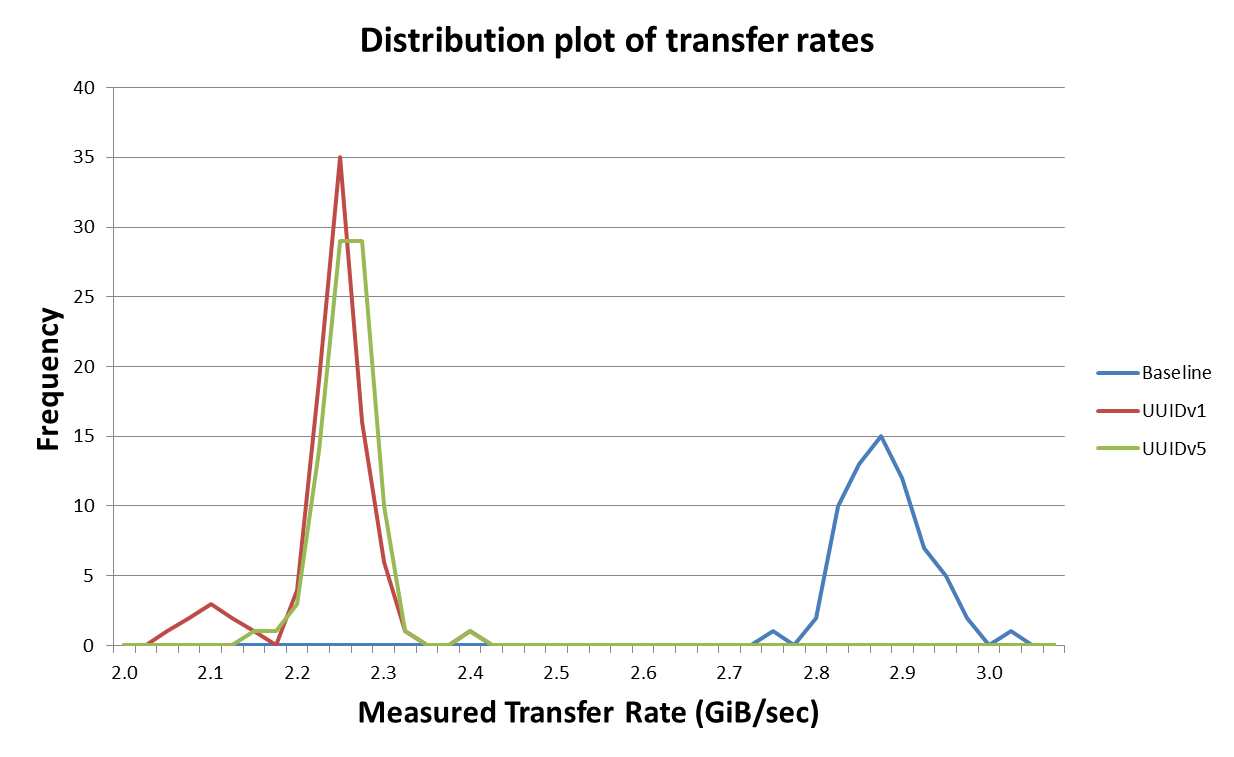
\includegraphics[width=\linewidth]{include/IPC-uuid-bench.png}
		\caption{Plot of the distribution of throughput values for each UUID generator. The shape of all 3 distributions is broadly similar, as would be expected, with an equal performance drop for both UUIDv1 and UUIDv5.}
		\label{fig:IPC-uuid-bench}
	\end{figure}
	
	As shown in Figure \ref{fig:IPC-uuid-bench}, the addition of UUID a generation algorithm did have a negative impact on performance, with a 20\% reduction in performance for both algorithms. There is little difference between the speed of the two algorithms, which is particularly surprising given how different they are in modus operandi.
	
	\subsection{Conclusion}
	
	From the results in Figure \ref{fig:IPC-uuid-bench}, there is clearly little to pick between the two UUID generation algorithms under consideration. However, this test was run with constant inputs to the v5 generator, and so the v5 system would still need some way of generating unique inputs. Doing so would likely involve implementing something similar to the v1 algorithm in our case, and so I chose to proceed using version 1 of the algorithm.
	
	
	\chapter{Implementation}
	
	\section{Kernel alterations}
	
	\subsection{Tagging packets with UUIDs}
	
	\subsection{Adding a kernel configuration option}
	
	\subsection{DTrace probes}
	
	\section{Core userspace datastructure - the `red-black trie'}
	
	\subsection{The datastructure}
	
	\subsection{Motivation}
	
	\subsection{Development approach}
	
	\section{Example application}
	
	\subsection{DTrace consumer}
	
	\subsection{Analysis API}
	
	\subsection{Front end}
	
	
	\chapter{Evaluation}
	
	
	\chapter{Conclusion}
	
	
	
	%%%%%%%%%%%%%%%%%%%%%%%%%%%%%%%%%%%%%%%%%%%%%%%%%%%%%%%%%%%%%%%%%%%%%
	% the bibliography
	\addcontentsline{toc}{chapter}{Bibliography}
	\bibliographystyle{plain}
	\bibliography{refs}
	
	%%%%%%%%%%%%%%%%%%%%%%%%%%%%%%%%%%%%%%%%%%%%%%%%%%%%%%%%%%%%%%%%%%%%%
	% the appendices
	\begin{appendices}
		\chapter{IPC Benchmark shell script}
		\label{appendix:IPC}
		
		The following shell script was used to execute the IPC benchmark 100 times to gather data on the throughput effects of the different UUID algorithms.
		
		\begin{verbatim}
		#!/bin/csh
		
		# First argument is ipc executable
		set ipc=$1
		# Second argument is csv file to output to
		set csv=$2
		
		# Overwrite any existing file with the header
		echo "Measured transfer rate" > $csv
		
		@ n = 0
		# Repeat the benchmark 100 times
		while ($n < 100)
		    # Allow the system to calm down before running benchmark
		    sleep 2
		    # 16GiB transfer is found to put the system under significant
		    # load for about 10 seconds, on my machine
		    $ipc -i tcp -t 17179869184 2proc | awk '{print $1}' >> $csv
		    @ n += 1
		end
		\end{verbatim}
	\end{appendices}
	
	
	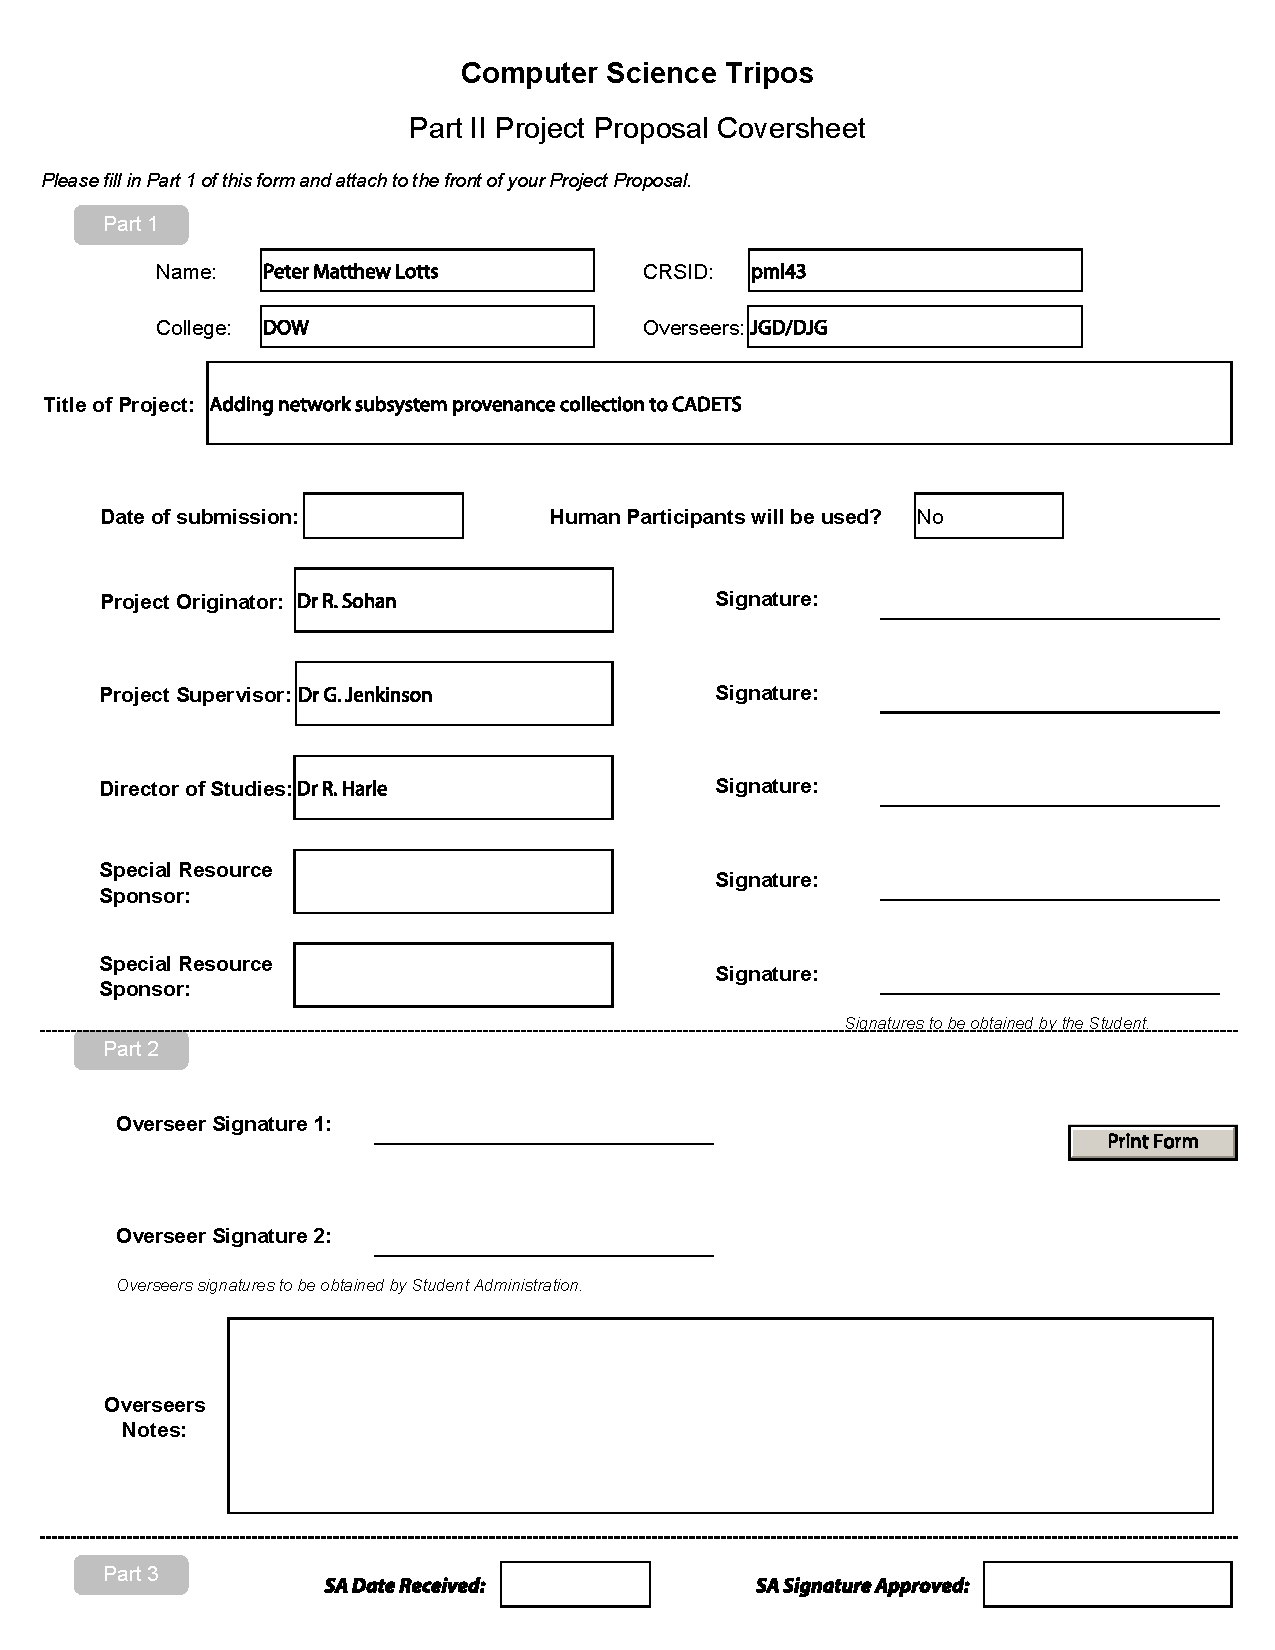
\includepdf{include/Project-Proposal-Cover-Sheet.pdf}
	\includepdf[pages={2-}]{include/Project-Proposal.pdf}
	
	
\end{document}
